\documentclass[twoside]{book}

% Packages required by doxygen
\usepackage{fixltx2e}
\usepackage{calc}
\usepackage{doxygen}
\usepackage[export]{adjustbox} % also loads graphicx
\usepackage{graphicx}
\usepackage[utf8]{inputenc}
\usepackage{makeidx}
\usepackage{multicol}
\usepackage{multirow}
\PassOptionsToPackage{warn}{textcomp}
\usepackage{textcomp}
\usepackage[nointegrals]{wasysym}
\usepackage[table]{xcolor}

% Font selection
\usepackage[T1]{fontenc}
\usepackage[scaled=.90]{helvet}
\usepackage{courier}
\usepackage{amssymb}
\usepackage{sectsty}
\renewcommand{\familydefault}{\sfdefault}
\allsectionsfont{%
  \fontseries{bc}\selectfont%
  \color{darkgray}%
}
\renewcommand{\DoxyLabelFont}{%
  \fontseries{bc}\selectfont%
  \color{darkgray}%
}
\newcommand{\+}{\discretionary{\mbox{\scriptsize$\hookleftarrow$}}{}{}}

% Page & text layout
\usepackage{geometry}
\geometry{%
  a4paper,%
  top=2.5cm,%
  bottom=2.5cm,%
  left=2.5cm,%
  right=2.5cm%
}
\tolerance=750
\hfuzz=15pt
\hbadness=750
\setlength{\emergencystretch}{15pt}
\setlength{\parindent}{0cm}
\setlength{\parskip}{3ex plus 2ex minus 2ex}
\makeatletter
\renewcommand{\paragraph}{%
  \@startsection{paragraph}{4}{0ex}{-1.0ex}{1.0ex}{%
    \normalfont\normalsize\bfseries\SS@parafont%
  }%
}
\renewcommand{\subparagraph}{%
  \@startsection{subparagraph}{5}{0ex}{-1.0ex}{1.0ex}{%
    \normalfont\normalsize\bfseries\SS@subparafont%
  }%
}
\makeatother

% Headers & footers
\usepackage{fancyhdr}
\pagestyle{fancyplain}
\fancyhead[LE]{\fancyplain{}{\bfseries\thepage}}
\fancyhead[CE]{\fancyplain{}{}}
\fancyhead[RE]{\fancyplain{}{\bfseries\leftmark}}
\fancyhead[LO]{\fancyplain{}{\bfseries\rightmark}}
\fancyhead[CO]{\fancyplain{}{}}
\fancyhead[RO]{\fancyplain{}{\bfseries\thepage}}
\fancyfoot[LE]{\fancyplain{}{}}
\fancyfoot[CE]{\fancyplain{}{}}
\fancyfoot[RE]{\fancyplain{}{\bfseries\scriptsize Generated by Doxygen }}
\fancyfoot[LO]{\fancyplain{}{\bfseries\scriptsize Generated by Doxygen }}
\fancyfoot[CO]{\fancyplain{}{}}
\fancyfoot[RO]{\fancyplain{}{}}
\renewcommand{\footrulewidth}{0.4pt}
\renewcommand{\chaptermark}[1]{%
  \markboth{#1}{}%
}
\renewcommand{\sectionmark}[1]{%
  \markright{\thesection\ #1}%
}

% Indices & bibliography
\usepackage{natbib}
\usepackage[titles]{tocloft}
\setcounter{tocdepth}{3}
\setcounter{secnumdepth}{5}
\makeindex

% Hyperlinks (required, but should be loaded last)
\usepackage{ifpdf}
\ifpdf
  \usepackage[pdftex,pagebackref=true]{hyperref}
\else
  \usepackage[ps2pdf,pagebackref=true]{hyperref}
\fi
\hypersetup{%
  colorlinks=true,%
  linkcolor=blue,%
  citecolor=blue,%
  unicode%
}

% Custom commands
\newcommand{\clearemptydoublepage}{%
  \newpage{\pagestyle{empty}\cleardoublepage}%
}

\usepackage{caption}
\captionsetup{labelsep=space,justification=centering,font={bf},singlelinecheck=off,skip=4pt,position=top}

%===== C O N T E N T S =====

\begin{document}

% Titlepage & ToC
\hypersetup{pageanchor=false,
             bookmarksnumbered=true,
             pdfencoding=unicode
            }
\pagenumbering{alph}
\begin{titlepage}
\vspace*{7cm}
\begin{center}%
{\Large Project V2 }\\
\vspace*{1cm}
{\large Generated by Doxygen 1.8.13}\\
\end{center}
\end{titlepage}
\clearemptydoublepage
\pagenumbering{roman}
\tableofcontents
\clearemptydoublepage
\pagenumbering{arabic}
\hypersetup{pageanchor=true}

%--- Begin generated contents ---
\chapter{Hierarchical Index}
\section{Class Hierarchy}
This inheritance list is sorted roughly, but not completely, alphabetically\+:\begin{DoxyCompactList}
\item \contentsline{section}{Dice}{\pageref{class_dice}}{}
\begin{DoxyCompactList}
\item \contentsline{section}{Scores}{\pageref{class_scores}}{}
\end{DoxyCompactList}
\item \contentsline{section}{dice\+Roll$<$ T $>$}{\pageref{classdice_roll}}{}
\item \contentsline{section}{Rules}{\pageref{class_rules}}{}
\item \contentsline{section}{scre\+Card}{\pageref{classscre_card}}{}
\end{DoxyCompactList}

\chapter{Class Index}
\section{Class List}
Here are the classes, structs, unions and interfaces with brief descriptions\+:\begin{DoxyCompactList}
\item\contentsline{section}{\hyperlink{struct_dice}{Dice} }{\pageref{struct_dice}}{}
\item\contentsline{section}{\hyperlink{structscre_card}{scre\+Card} }{\pageref{structscre_card}}{}
\end{DoxyCompactList}

\chapter{Class Documentation}
\hypertarget{class_dice}{}\section{Dice Class Reference}
\label{class_dice}\index{Dice@{Dice}}
Inheritance diagram for Dice\+:\begin{figure}[H]
\begin{center}
\leavevmode
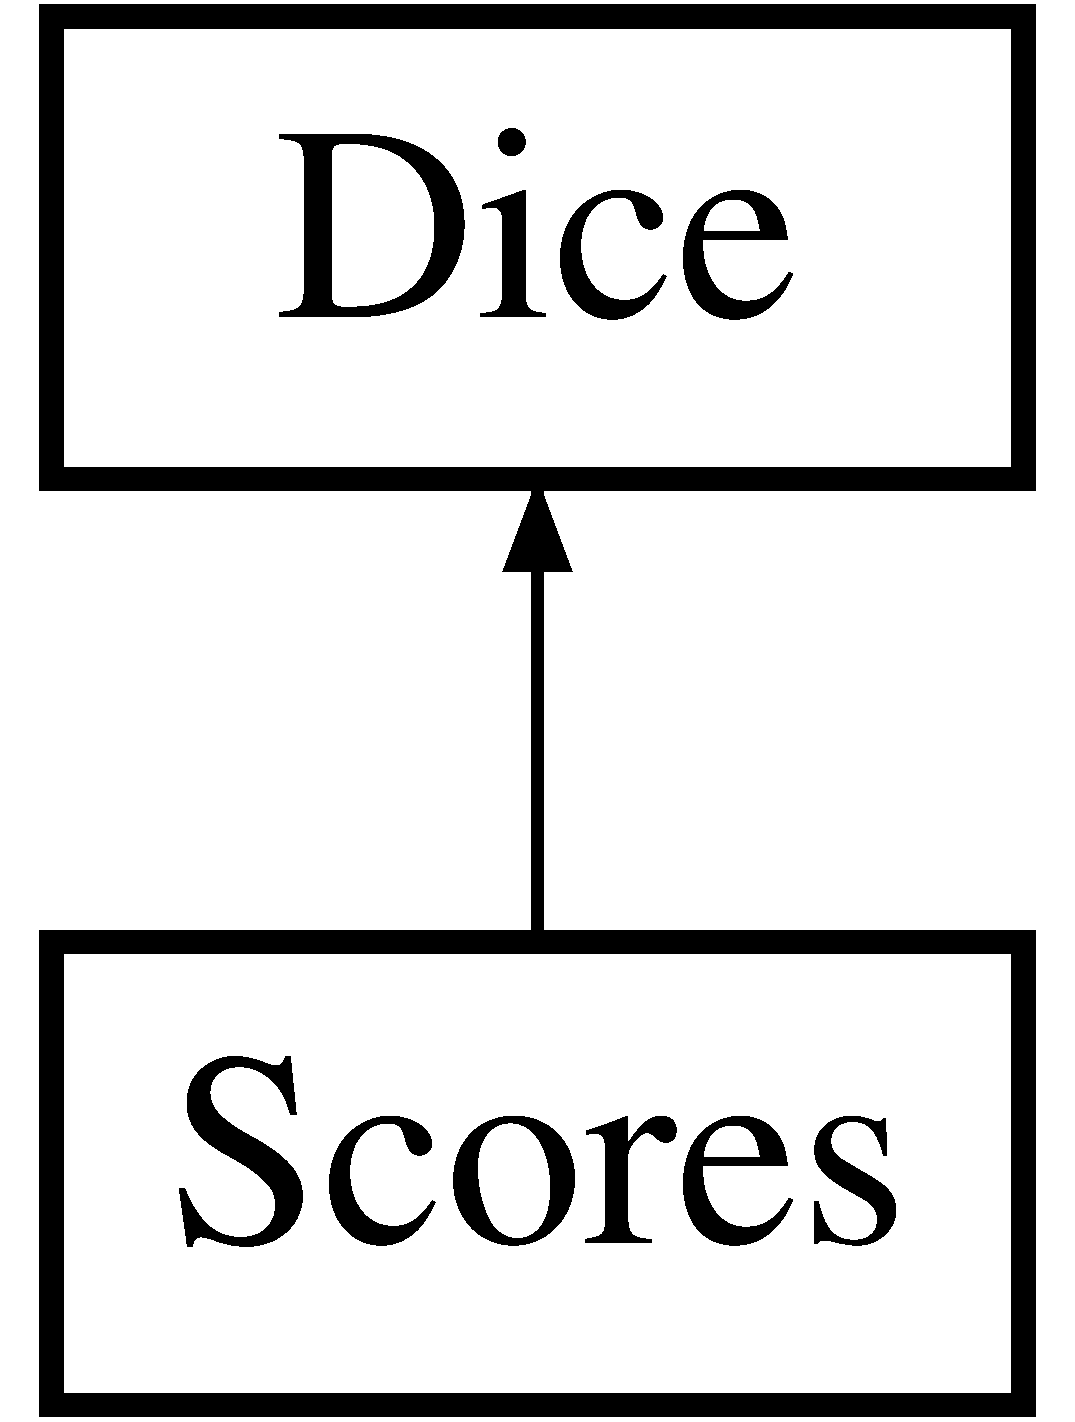
\includegraphics[height=2.000000cm]{class_dice}
\end{center}
\end{figure}
\subsection*{Public Member Functions}
\begin{DoxyCompactItemize}
\item 
\mbox{\Hypertarget{class_dice_aa1d3bf588284f83cb45f4b284ebcc748}\label{class_dice_aa1d3bf588284f83cb45f4b284ebcc748}} 
virtual void {\bfseries print} ()
\end{DoxyCompactItemize}
\subsection*{Public Attributes}
\begin{DoxyCompactItemize}
\item 
\mbox{\Hypertarget{class_dice_ae1c369fc5164bac7ec31d7a6d5d7df1d}\label{class_dice_ae1c369fc5164bac7ec31d7a6d5d7df1d}} 
int {\bfseries dice1}
\item 
\mbox{\Hypertarget{class_dice_aaa67d915e4554b1c862f7ee0a9afff8c}\label{class_dice_aaa67d915e4554b1c862f7ee0a9afff8c}} 
int {\bfseries dice2}
\item 
\mbox{\Hypertarget{class_dice_a49752c1eca2817629d0406b595fd4b56}\label{class_dice_a49752c1eca2817629d0406b595fd4b56}} 
int {\bfseries dice3}
\item 
\mbox{\Hypertarget{class_dice_aeca1db89c9f2d16d94a0b3c7b0b9ca1c}\label{class_dice_aeca1db89c9f2d16d94a0b3c7b0b9ca1c}} 
int {\bfseries dice4}
\item 
\mbox{\Hypertarget{class_dice_ac0e5ca3b8134775f129c34ed9c6d616a}\label{class_dice_ac0e5ca3b8134775f129c34ed9c6d616a}} 
int {\bfseries dice5}
\item 
\mbox{\Hypertarget{class_dice_a86b43ccbc36a292a01f78219be7f0484}\label{class_dice_a86b43ccbc36a292a01f78219be7f0484}} 
int {\bfseries dice6}
\end{DoxyCompactItemize}


The documentation for this class was generated from the following files\+:\begin{DoxyCompactItemize}
\item 
C\+:/\+Users/\+Andrew/\+Desktop/\+Project 2 V2/\+Project 2 V2/dice.\+h\item 
C\+:/\+Users/\+Andrew/\+Desktop/\+Project 2 V2/\+Project 2 V2/dice.\+cpp\end{DoxyCompactItemize}

\hypertarget{classdice_roll}{}\section{dice\+Roll$<$ T $>$ Class Template Reference}
\label{classdice_roll}\index{dice\+Roll$<$ T $>$@{dice\+Roll$<$ T $>$}}
\subsection*{Public Member Functions}
\begin{DoxyCompactItemize}
\item 
\mbox{\Hypertarget{classdice_roll_acabe620a4ddacc7c95c3ec3cdaf87e92}\label{classdice_roll_acabe620a4ddacc7c95c3ec3cdaf87e92}} 
{\bfseries roll} (int)
\end{DoxyCompactItemize}
\subsection*{Private Attributes}
\begin{DoxyCompactItemize}
\item 
\mbox{\Hypertarget{classdice_roll_a02f17349ce7d83129bf01297ce86148e}\label{classdice_roll_a02f17349ce7d83129bf01297ce86148e}} 
T $\ast$ {\bfseries data}
\end{DoxyCompactItemize}


The documentation for this class was generated from the following file\+:\begin{DoxyCompactItemize}
\item 
C\+:/\+Users/\+Andrew/\+Desktop/\+Project 2 V2/\+Project 2 V2/dice.\+h\end{DoxyCompactItemize}

\hypertarget{class_rules}{}\section{Rules Class Reference}
\label{class_rules}\index{Rules@{Rules}}
\subsection*{Public Member Functions}
\begin{DoxyCompactItemize}
\item 
\mbox{\Hypertarget{class_rules_a1c81df7f15aa63713f7b7b1ddff802d7}\label{class_rules_a1c81df7f15aa63713f7b7b1ddff802d7}} 
void {\bfseries shw\+Cntnts} (fstream \&file)
\end{DoxyCompactItemize}
\subsection*{Private Attributes}
\begin{DoxyCompactItemize}
\item 
\mbox{\Hypertarget{class_rules_a4139c3a5420a8ecccd5b9caafc1d77a4}\label{class_rules_a4139c3a5420a8ecccd5b9caafc1d77a4}} 
string {\bfseries line}
\end{DoxyCompactItemize}


The documentation for this class was generated from the following files\+:\begin{DoxyCompactItemize}
\item 
C\+:/\+Users/\+Andrew/\+Desktop/\+Project 2 V2/\+Project 2 V2/rules.\+h\item 
C\+:/\+Users/\+Andrew/\+Desktop/\+Project 2 V2/\+Project 2 V2/rules.\+cpp\end{DoxyCompactItemize}

\hypertarget{class_scores}{}\section{Scores Class Reference}
\label{class_scores}\index{Scores@{Scores}}
Inheritance diagram for Scores\+:\begin{figure}[H]
\begin{center}
\leavevmode
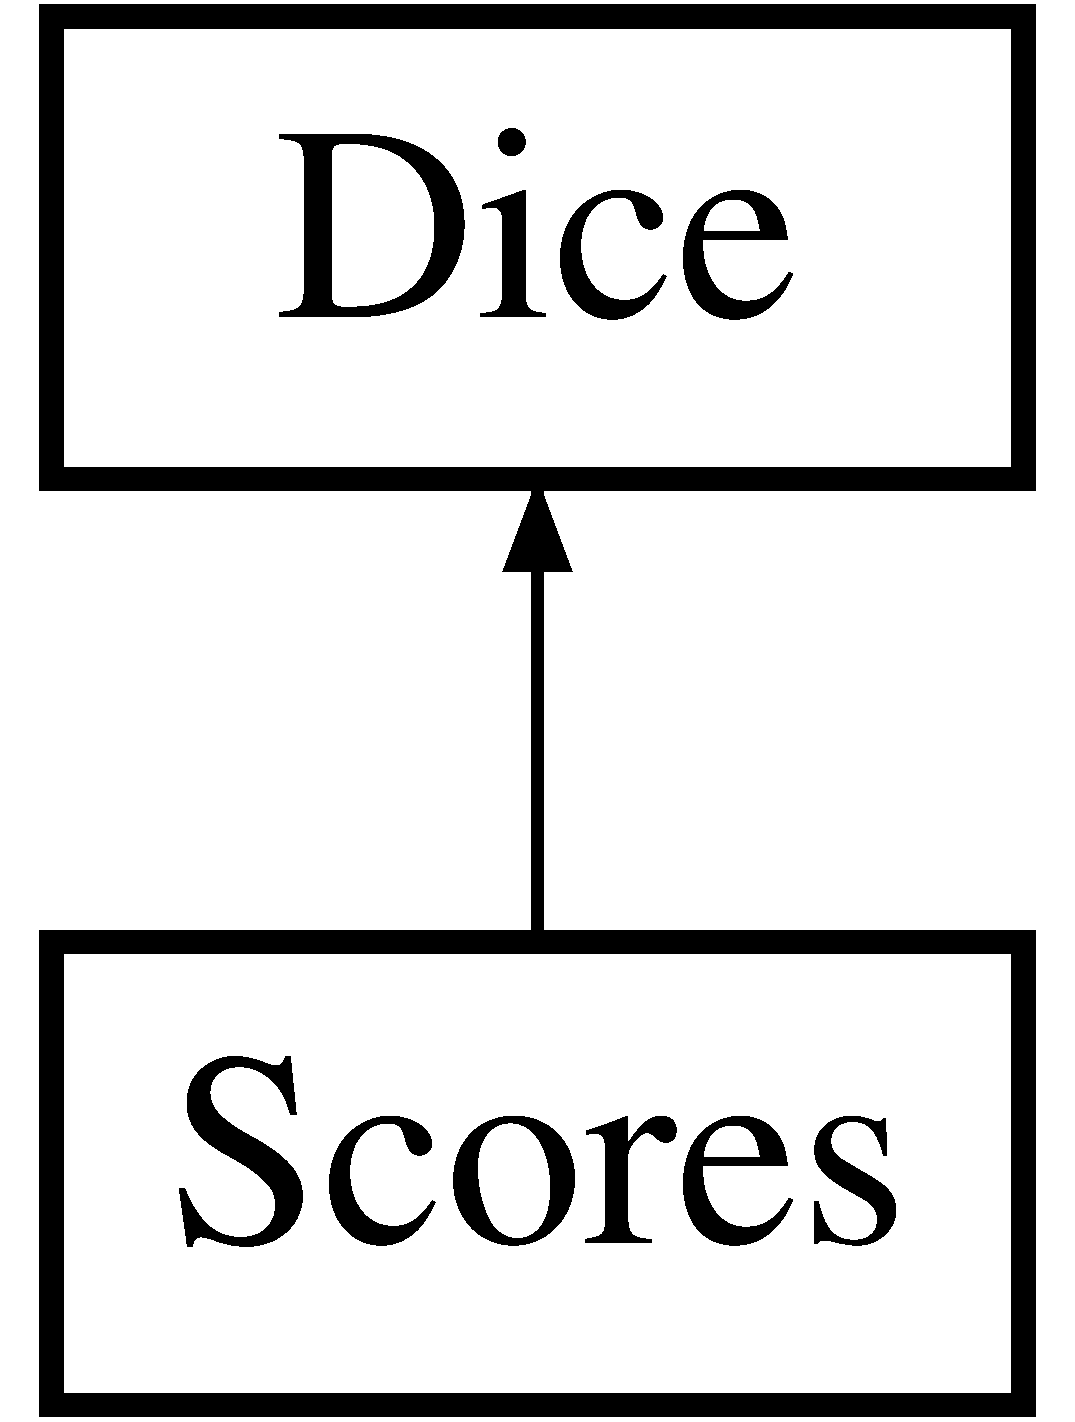
\includegraphics[height=2.000000cm]{class_scores}
\end{center}
\end{figure}
\subsection*{Public Member Functions}
\begin{DoxyCompactItemize}
\item 
\mbox{\Hypertarget{class_scores_a0c8e4646e9f50403e07dc8348266edee}\label{class_scores_a0c8e4646e9f50403e07dc8348266edee}} 
void {\bfseries roll\+Scres} ()
\item 
\mbox{\Hypertarget{class_scores_ac46f2819ee979baecd75180b47753bbe}\label{class_scores_ac46f2819ee979baecd75180b47753bbe}} 
void {\bfseries print} ()
\end{DoxyCompactItemize}
\subsection*{Additional Inherited Members}


The documentation for this class was generated from the following files\+:\begin{DoxyCompactItemize}
\item 
C\+:/\+Users/\+Andrew/\+Desktop/\+Project 2 V2/\+Project 2 V2/dice.\+h\item 
C\+:/\+Users/\+Andrew/\+Desktop/\+Project 2 V2/\+Project 2 V2/dice.\+cpp\end{DoxyCompactItemize}

\hypertarget{classscre_card}{}\section{scre\+Card Class Reference}
\label{classscre_card}\index{scre\+Card@{scre\+Card}}
\subsection*{Public Member Functions}
\begin{DoxyCompactItemize}
\item 
\mbox{\Hypertarget{classscre_card_a85c6f2e648561d4044d034c96664c5b6}\label{classscre_card_a85c6f2e648561d4044d034c96664c5b6}} 
void {\bfseries scre\+Board} (\hyperlink{classscre_card}{scre\+Card} $\ast$scre)
\end{DoxyCompactItemize}
\subsection*{Protected Attributes}
\begin{DoxyCompactItemize}
\item 
\mbox{\Hypertarget{classscre_card_a142a055fa3894891503722f06c691a4d}\label{classscre_card_a142a055fa3894891503722f06c691a4d}} 
char {\bfseries name} \mbox{[}$\,$\mbox{]}
\item 
\mbox{\Hypertarget{classscre_card_aca36017ce3ff1201a38b9c975c20d242}\label{classscre_card_aca36017ce3ff1201a38b9c975c20d242}} 
int {\bfseries one}
\item 
\mbox{\Hypertarget{classscre_card_a5d802886236a00e701bb68c5ba7de71e}\label{classscre_card_a5d802886236a00e701bb68c5ba7de71e}} 
int {\bfseries two}
\item 
\mbox{\Hypertarget{classscre_card_a44b505ee324fb103931d5a1e2ce9b5d1}\label{classscre_card_a44b505ee324fb103931d5a1e2ce9b5d1}} 
int {\bfseries three}
\item 
\mbox{\Hypertarget{classscre_card_ad9586f49eeb39857826c114c5c1a65cb}\label{classscre_card_ad9586f49eeb39857826c114c5c1a65cb}} 
int {\bfseries four}
\item 
\mbox{\Hypertarget{classscre_card_a39fb932db642a35d5dd156045dea5c62}\label{classscre_card_a39fb932db642a35d5dd156045dea5c62}} 
int {\bfseries five}
\item 
\mbox{\Hypertarget{classscre_card_ae82cf09db1ccd36380a509f240b71040}\label{classscre_card_ae82cf09db1ccd36380a509f240b71040}} 
int {\bfseries six}
\item 
\mbox{\Hypertarget{classscre_card_a5af84c119b4f58da73e851e18dfb7ae6}\label{classscre_card_a5af84c119b4f58da73e851e18dfb7ae6}} 
int {\bfseries thr\+Kind}
\item 
\mbox{\Hypertarget{classscre_card_ac76f9907ba8e2795968cd06042a98c42}\label{classscre_card_ac76f9907ba8e2795968cd06042a98c42}} 
int {\bfseries four\+Kind}
\item 
\mbox{\Hypertarget{classscre_card_a4a2ecf756a6e0bc87e4e049941ab40e9}\label{classscre_card_a4a2ecf756a6e0bc87e4e049941ab40e9}} 
int {\bfseries ful\+Huse}
\item 
\mbox{\Hypertarget{classscre_card_a7c159f368baece5e9486c95a17243f52}\label{classscre_card_a7c159f368baece5e9486c95a17243f52}} 
int {\bfseries sml\+Strght}
\item 
\mbox{\Hypertarget{classscre_card_a337ee925dc5831958deb35df999272de}\label{classscre_card_a337ee925dc5831958deb35df999272de}} 
int {\bfseries lrge\+Strght}
\item 
\mbox{\Hypertarget{classscre_card_a51c57ac55b54259138ee5050737870f3}\label{classscre_card_a51c57ac55b54259138ee5050737870f3}} 
int {\bfseries chnce}
\item 
\mbox{\Hypertarget{classscre_card_a8e09c3ec5e587e509d328af285e028b8}\label{classscre_card_a8e09c3ec5e587e509d328af285e028b8}} 
int {\bfseries yhtze}
\item 
\mbox{\Hypertarget{classscre_card_abbef5f6461fd43f42b5cbc3d80201965}\label{classscre_card_abbef5f6461fd43f42b5cbc3d80201965}} 
int {\bfseries ttl}
\item 
\mbox{\Hypertarget{classscre_card_a3d1894a3cb33c1dddca4488f5b24d3aa}\label{classscre_card_a3d1894a3cb33c1dddca4488f5b24d3aa}} 
int {\bfseries sum}
\item 
\mbox{\Hypertarget{classscre_card_a236a10cc04262b34ec7f451ce48d6601}\label{classscre_card_a236a10cc04262b34ec7f451ce48d6601}} 
int {\bfseries bnus}
\item 
\mbox{\Hypertarget{classscre_card_a8a26609e3af7188b3de9aafdfbfe7322}\label{classscre_card_a8a26609e3af7188b3de9aafdfbfe7322}} 
int {\bfseries roll}
\item 
\mbox{\Hypertarget{classscre_card_a110c480d7941945972c62ec1858b3ce8}\label{classscre_card_a110c480d7941945972c62ec1858b3ce8}} 
int {\bfseries amnt}
\item 
\mbox{\Hypertarget{classscre_card_acad4ba6ad4d766bbdb27529f24bfcf76}\label{classscre_card_acad4ba6ad4d766bbdb27529f24bfcf76}} 
int {\bfseries yaht}
\end{DoxyCompactItemize}
\subsection*{Static Protected Attributes}
\begin{DoxyCompactItemize}
\item 
\mbox{\Hypertarget{classscre_card_a485879ffa922530b13036a5078913e4a}\label{classscre_card_a485879ffa922530b13036a5078913e4a}} 
static const int {\bfseries size} =50
\end{DoxyCompactItemize}


The documentation for this class was generated from the following files\+:\begin{DoxyCompactItemize}
\item 
C\+:/\+Users/\+Andrew/\+Desktop/\+Project 2 V2/\+Project 2 V2/scre\+Card.\+h\item 
C\+:/\+Users/\+Andrew/\+Desktop/\+Project 2 V2/\+Project 2 V2/scre\+Card.\+cpp\end{DoxyCompactItemize}

%--- End generated contents ---

% Index
\backmatter
\newpage
\phantomsection
\clearemptydoublepage
\addcontentsline{toc}{chapter}{Index}
\printindex

\end{document}
